\documentclass[titlepage = firstcover]{scrartcl}
\usepackage[aux]{rerunfilecheck}
\usepackage{fontspec}
\usepackage[main=ngerman, english, french]{babel}

% mehr Pakete hier
\usepackage{expl3}
\usepackage{xparse}
\usepackage{pdfpages}

%Mathematik------------------------------------------------------
\usepackage{amsmath}   % unverzichtbare Mathe-Befehle
\usepackage{amssymb}   % viele Mathe-Symbole
\usepackage{mathtools} % Erweiterungen für amsmath
\usepackage[
  math-style=ISO,    % \
  bold-style=ISO,    % |
  sans-style=italic, % | ISO-Standard folgen
  nabla=upright,     % |
  partial=upright,   % /
]{unicode-math}% "Does exactly what it says on the tin."
\usepackage[section, below]{placeins}
\usepackage{upgreek}

% Laden von OTF-Mathefonts
% Ermöglich Unicode Eingabe von Zeichen: α statt \alpha

\setmathfont{Latin Modern Math}
%\setmathfont{Tex Gyre Pagella Math} % alternativ zu Latin Modern Math
\setmathfont{XITS Math}[range={scr, bfscr}]
\setmathfont{XITS Math}[range={cal, bfcal}, StylisticSet=1]

\AtBeginDocument{ % wird bei \begin{document}
  % werden sonst wieder von unicode-math überschrieben
  \RenewDocumentCommand \Re {} {\operatorname{Re}}
  \RenewDocumentCommand \Im {} {\operatorname{Im}}
}
\usepackage{mleftright}
\setlength{\delimitershortfall}{-1sp}

%Sprache----------------------------------------------------------
\usepackage{microtype}
\usepackage{xfrac}
\usepackage[autostyle]{csquotes}    % babel
\usepackage[unicode, pdfusetitle]{hyperref}
\usepackage{bookmark}
\usepackage[shortcuts]{extdash}
%Einstellungen hier, z.B. Fonts
\usepackage{booktabs} % Tabellen
\usepackage{a4}
\usepackage{float}

\setlength{\parindent}{0pt}


\title{Compton-Effekt}
\author{David Gutnikov \\
        \href{mailto:david.gutnikov@tu-dortmund.de}{david.gutnikov@tu-dortmund.de}}
\date{Abgabe am 04.05.2020}


\begin{document}

    \maketitle
    \newpage
    \tableofcontents
    \newpage

    \section{Theorie}
      Die Streuung von Röntgenstrahlen an Materie wird in zwei Arten unterteilt: In die kohärente bzw. inelastische Streuung und in die inkohärente bzw. elastische frequenzverschobene Streuung. Dieser Versuch setzt sich mit der ersten Art der Streuung, der Compton-Streuung auseinander. Dabei trifft ein Photon der Wellenlänge $\lambda_1$ auf ein freies Elektron in der Materie, überträgt dem Elektron einen Teil seiner Energie, wird um einen Winkel $\theta$ von seiner ursprünglichen Richtung abgelenkt und besitzt die Wellenlänge $\lambda_2$.
      \begin{figure}[h]
        \centering
        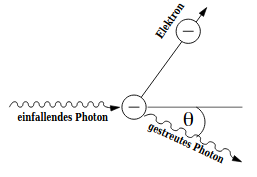
\includegraphics[width = 0.35\linewidth]{ComptoneffektSkizze.png}
        \caption{Vereinfachte Darstellung des Compton-Effektes}
        \label{fig:comptoneffekt}
      \end{figure}
      \FloatBarrier

      Die Wellenlängendifferenz $\Updelta\lambda = \lambda_2 - \lambda_1$ wird nach folgender Formel bestimmt
      \begin{equation}
        \Updelta\lambda = \frac{h}{m_e c}\bigl(1 - \cos{\theta}\bigr)
        \label{eqn:compton}
      \end{equation}
      mit dem Plankschen Wirkungsquantum $h$, der Lichtgeschwindigkeit $c$ und der Elektronenmasse $m_e$. Die Compton-Wellenlänge wird als $\lambda_\text{C} = h / (m_e c)$ definiert. Es ist leicht zu erkennen, dass die Wellenlängendifferenz bei $\theta = 180°$ mit $\Updelta\lambda = 2\lambda_\text{C}$ maximal und bei $\theta = 0°$ mit $\Updelta\lambda = 0$ minimal ist.

      In diesem Versuch wird die Compton-Wellenlänge indirekt durch das Transmissionsverhalten der Röntgenstrahlung bestimmt, weshalb ein paar Grundkenntnisse zu Röntgenstrahlung und Transmission gebraucht werden.

      \subsection{Röntgenstrahlung}
        Um Röntgenstrahlung zu erzeugen werden in einer evakuierten Röhre Elektronen aus einer Glühkathode gelöst und mithilfe einer Anode beschleunigt. Die herausgelösten Elektronen treffen auf das Anodenmaterial und verursachen Röntgenstrahlung.

        Das Röntgenspektrum setzt sich aus zwei Strahlungsarten zusammen, der kontinuirlichen Bremsstrahlung und der charakteristischen Röntgenstrahlung.

        Auslöser für die kontinuirliche Bremsstrahlung ist die Abbremsung eines Elektrons im elektrischen Feld eines Atoms des Anodenmaterials. Es wrid ein Photon ausgesandt, dessen Energie dem Energieverlust des Elektrons entspricht. Da die kinetische Energie eines Elektrons kontinuirlich ist, ist auch die Energie des erzeugten Photons und somit die Bremsstrahlung kontinuirlich.

        Die auftreffenden Elektronen regen Atome im Anodenmaterial an, d.h. Elektronen in den äußeren Schalen werden auf höhere Energieniveaus gehoben. Nach kurzer Zeit fallen die angeregten Elektronen wieder auf ein niedrigeres Energieniveau zurück, wobei ein Röntgenquant, dessen Energie der Eniergiediffenrenz zwischen den beiden Energieniveaus entspricht, emmitiert wird. Diese Energiedifferenz kann nur quantisierte Werte annehmen, weshalb auch die Photonen, also die Strahlung nur charakteristische Werte hat.

      \subsection{Absorption}
        Die Absorption eines Materials hängt hauptsächlich von drei wichtigen Prozessen ab, dem Photoeffekt, der Paarbildung und dem Compton-Effekt. Also setzt sich der stoffabhängige Absorptionskoeffizient $\mu = \mu_\text{Ph} + \mu_\text{Pa} + \mu_\text{Co}$ eines Materials aus dem Absorptionskoeffizienten des Photoeffektes $\mu_\text{Ph}$, der Paarbildung $\mu_\text{Pa}$ und des Comtpton-Effektes $\mu_\text{Co}$ zusammen. Für die Intensität der Strahlung $I$, die durch eine Materie der Dicke $d$ transmittiert ist, gilt mit der Intensität vor der Transmission $I_0$:
        \begin{equation*}
          I = I_0 e^{-\mu d}
        \end{equation*}
        Der Absorptionskoeffizient ist außerdem energieabhängig. Je kleiner die Energie des Photons / je größer seine Wellenlänge, desto größer der Absorptionskoeffizient. Im Bereich der Röntgenstrahlung $E \approx 1$ -$100$keV sind die beiden anderen Absorptionskoeffizienten zu vernachlässigen, sodass ca. für den Gesamtabsorptionskoeffizienten gilt: $\mu \approx \mu_\text{Co}$.

      \subsection{Bragg-Reflexion}
        Die Bragg-Bedingung besagt bei welchem Winkel $\alpha$ es zu einer konstruktiven Interferenz von Wellen bei einer Streuung an einem Gitter kommt. Treffen Photonen auf einen Kristall, also auf ein Gitter aus Atomen, wird ein kleiner Teil der Photonen an den Gitterebenen gebeugt. Doch diese Reflexion ist nur dann nennenswert, wenn die einzelnen reflektierten Anteile aus den verschiedenen Gitterebenen konstruktiv interferieren. Es muss deshalb für die Wellenlänge $\lambda$, den Netzebenenabstand $d$, die Glanzwinkel $\alpha$ und die Ordnung des Maximums der konstruktiven Interferenz $n$ die Bragg-Bedingung gelten:
        \begin{equation}
          n \lambda = 2 d \sin{\alpha}
          \label{eqn:bragg}
        \end{equation}

      \subsection{Totzeitkorrektur}
        Die Totzeit ist die Zeit, in der ein Gerät nach Registrierung eines Teilchens keine weiteren Teilchen registrieren kann. Wenn also ein zweites Teilchen in den Apparat fliegt bevor die Totzeit abgeklungen ist, werden die zwei Teilchen als Eins gezählt.
        Es gibt zwei verschiedene Arten von Totzeit, die nicht verlängerbare und die verlängerbare Totzeit.
        Beim Geiger-Müller-Zählrohr geht es um die nicht verlängerbare Totzeit. Dabei fängt eine nächste Totzeit nur an, wenn die vorherige Totzeit zuende gegangen ist.

        Für zur Totzeit vergleichsweise hochfrequente Ereignisse gilt, dass der Anteil der der Gesamttotzeit an der Messdauer dem Anteil der durch die Totzeit verlorenen Ereignisse entspricht
        \begin{align}
          \frac{n^* - n}{n} = \frac{N\tau}{T} \quad & \implies \quad 1 - \frac{n}{n^*} = \frac{N\tau}{\frac{N}{n}} \\
          \implies \quad n^* & = \frac{n}{1 - n\tau}
          \label{eqn:totzeitkorrektur}
        \end{align}
        mit der Messrate $n$, der tatsächlichen Messrate $n^*$, der Totzeit $\tau$, der Anzahl der gemessenen Ereignisse $N$ und der Messdauer $T = N / n$.

      \section{Aufbau und Durchführung}
        \subsection{Aufnahme des Emissionsspektrum der Kupfer-Anode}
          Hierbei wird eine 2mm-Blende verwendet um die Röntgenstrahlung, die aus der Kupferanode austritt zu fokussieren. Die Röntgenstrahlung trifft auf einen LiF-Kristall hinter dem ein Geiger-Müller-Zählrohr angebracht ist. Dieser Kristall und das Zählrohr werden nach jeder Messung in 0.2° Schritten gedreht.

        \subsection{Aufnahme der Transmissionkurve}
          Für diese Messung wird der LiF-Kristall in einem Winkelbereich von 7° bis 10° in 0.1° Schritten gedreht. Es werden zwei Messreihen aufgenommen, einmal die Zähleraten ohne Absorber $n_0$ und einmal die Zählraten mit einem Aluminium-Absorber vor der 2mm-Blende $n_\textup{Al}$.

        \subsection{Messungen der durch Compton-Streuung ausgelösten Röntgenquanten} \label{messungen}
          \begin{figure}[h]
            \centering
            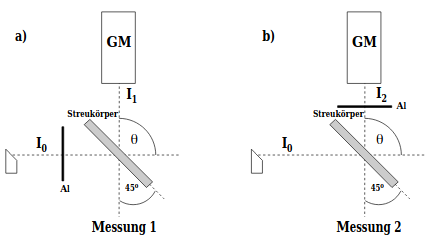
\includegraphics[width = 0.6\linewidth]{Compton_Aufbau.png}
            \caption{Aufbau des Versuchs zur Bestimmung der Comtpton-Wellenlänge}
            \label{fig:aufbau}
          \end{figure}
          \FloatBarrier
          
          Die 2mm-Blende wird durch eine 5mm-Blende und der LiF-Kristall wird durch einen Plexiglas-Streuer ersetzt. Der Streuer wird auf 45° und das Geiger-Müller-Zählrohr wird auf 90° ausgerichtet wie es in \ref{fig:aufbau} zu sehen ist. Jetzt wird die Intensität ohne Absorber $I_0$, die Intensität mit dem Aluminium-Absober zwischen Blende und Streuer $I_1$ und die Intensität mit dem Aluminium-Absorber zwischen Streuer und Zählrohr $I_2$ gemessen.
      
      \section{Auswertung}
        \subsection{Emissionsspektrum der Kupfer-Anode}
        \begin{figure}[h]
          \centering
          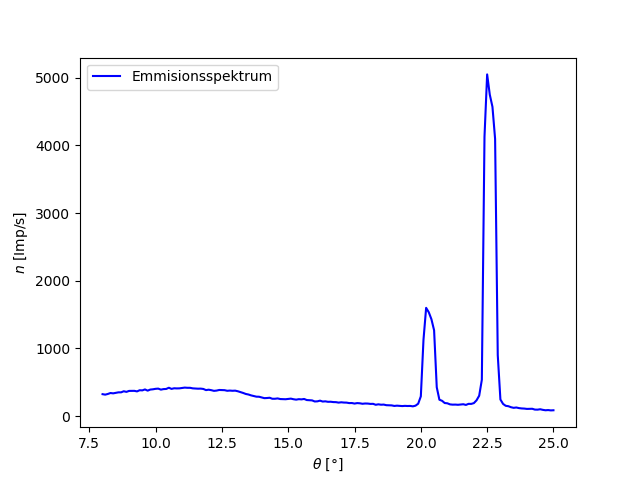
\includegraphics[width = 0.8\linewidth]{EmissionCu.png}
          \caption{Röntegenspektrum der Kupferanode aus der Tabelle \ref{tab:emission}}
          \label{fig:emission}
        \end{figure}
        \FloatBarrier
        
        Die $K_{\alpha}$-Linie und die $K_{\beta}$-Linie sind in \ref{fig:emission} deutlich zu erkennen. Es lässt lassen sich ca. die Werte $\theta_{\alpha} = 22.5$ und $\theta_{\beta} = 20.3$ für die Winkel der Peaks bestimmen. Somit kommt man mit \ref{eqn:bragg} und mit $E = hc/\lambda$ auf die Energiewerte $E_{\alpha} = 8,043$ keV und $E_{\beta} = 8,872$ keV für die $K_{\alpha}$-Linie und die $K_{\beta}$-Linie.

        Mit den wahren Energiewerten $E_{\alpha\text{,wahr}} = 8,038$ keV und $E_{\beta\text{,wahr}} = 8,905$ keV ergeben sich relative Abweichungen von $a_{\alpha} = 0,067\%$ und $a_{\beta} = 0,37\%$.

      \subsection{Transmissionskurve}
        Die Winkel in \ref{fig:transmissionstabelle} werden mit der Bragg-Gleichung \ref{eqn:bragg} in die zugehörigen Wellenlängen umgewandelt. Die Zählraten $n_0$ und $n_\text{Al}$ werden nach \ref{eqn:totzeitkorrektur} korrigiert. Aus den korrigierten Zählraten $n_0^*$ und $n_\text{Al}^*$ wird mit $T = n_\text{Al}^* / n_0^*$ die Transmission berechnet und gegen die Wellenlänge aufgetragen.
        \begin{figure}[h]
          \centering
          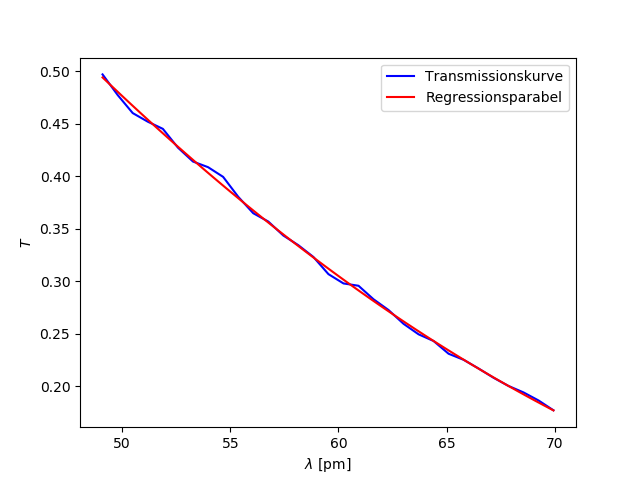
\includegraphics[width = 0.8\linewidth]{Transmissionskurve.png}
          \caption{Der Graph zeigt die Transmission der Strahlung gegen ihre Wellenlänge aufgetragen. Es wird auch eine Regressionsparabel zu den Punkten angezeigt.}
          \label{fig:transmissionskurve}
        \end{figure}
        \FloatBarrier

        Die Regressionsparabel hat die Form:
        \begin{equation*}
          f(x) = ax^2 + bx + c
        \end{equation*}
        mit den Parameter:
        \begin{align*}
          a &= (2,14 \pm 0,17) \cdot 10^{-4} \\
          b &= (-4,07 \pm 0,20) \cdot 10^{-2} \\
          c &= (1,97 \pm 0,06)
        \end{align*}
        
      \subsection{Bestimmung der Compton-Wellenlänge}
        Mit den Werten aus den Messungen \ref{messungen} wird die Transmission für die noch nicht gestreute Röntgenstrahlung $T_1 = I_2 / I_0$ und die Transmission für die gestreute Röntgenstrahlung $T_1 = I_2 / I_0$ bestimmt.
        \begin{align*}
          I_0 = 2731 \quad \text{Impulse}\\
          I_1 = 1180 \quad \text{Impulse}\\
          I_2 = 1024 \quad \text{Impulse}
        \end{align*}
        Es ergeben sich die Werte:
        \begin{align*}
          T_1 = 0,4321\\
          T_2 = 0,3750
        \end{align*}
        Die Werte für die Wellenlängen $\lambda_1$ und $\lambda_2$ werden aus der Regressionsparabel für die Transmissionskurve bestimmt.
        \begin{align*}
          \lambda_1 &= 52,37 \, \text{pm}\\
          \lambda_2 &= 55,62 \, \text{pm}
        \end{align*}
        Da das Geiger-Müller-Zählrohr im 90°-Winkel aufgestellt ist, gilt für die Compton-Wellenlänge nach \ref{fig:comptoneffekt}:
        \begin{equation*}
          \lambda_\text{C} = \lambda_2 - \lambda_1 = 3,25 \, \text{pm}
        \end{equation*}
        Mit der Compton-Wellenlänge eines Elektron aus der Literatur $\lambda_\text{C,wahr} = 2,4263$ pm entsteht eine relative Abweichung von ca. $25,41\%$.

      \section{Diskussion}
        Bei geringeren Zählraten ist keine Totzeitkorrektur nötig, da sie das Ergebnis nicht mehr korregieren, sondern verfälschen würde. Ist die Totzeitdauer im Vergleich zur durchschnittlichen Dauer bis ein Ereignis eintritt sehr klein, so würde ein Ereignis nur mit einer sehr kleinen Wahrscheinlichkeit in in der Totzeit landen. Damit würde man mit der Totzeitkorrektur die Zählrate niedriger schätzen als sie eigentlich ist.

        Es gibt den systematischen Fehler, dass auch am Aluminium-Absorber der Compton-Effekt auftreten und ins Zählrohr gelangen kann.
      
      \section{Daten}
        \begin{table}
          \centering
          \caption{Die Werte für den Winkel und die Zählraten für das Röntgensprektrum.}
          \label{tab:emission}
          \begin{tabular}{c c c c c c c c}
            \toprule
            $\theta$ [°] & $n$ [Imp/s] & $\theta$ [°] & $n$ [Imp/s] & $\theta$ [°] & $n$ [Imp/s] & $\theta$ [°] & $n$ [Imp/s] \\
            \midrule                                                         
            8.0	 & 323.0 & 12.3 & 376.0 & 16.6 & 211.0 &  20.9 & 192.0\\ 
            8.1	 & 316.0 & 12.4 & 385.0 & 16.7 & 206.0 &  21.0 & 188.0\\ 
            8.2	 & 326.0 & 12.5 & 384.0 & 16.8 & 205.0 &  21.1 & 172.0\\ 
            8.3	 & 340.0 & 12.6 & 382.0 & 16.9 & 198.0 &  21.2 & 168.0\\ 
            8.4	 & 335.0 & 12.7 & 373.0 & 17.0 & 203.0 &  21.3 & 169.0\\ 
            8.5	 & 343.0 & 12.8 & 376.0 & 17.1 & 199.0 &  21.4 & 166.0\\ 
            8.6	 & 350.0 & 12.9 & 373.0 & 17.2 & 198.0 &  21.5 & 170.0\\ 
            8.7	 & 350.0 & 13.0 & 375.0 & 17.3 & 191.0 &  21.6 & 174.0\\ 
            8.8	 & 366.0 & 13.1 & 366.0 & 17.4 & 192.0 &  21.7 & 164.0\\ 
            8.9	 & 357.0 & 13.2 & 354.0 & 17.5 & 184.0 &  21.8 & 180.0\\ 
            9.0	 & 371.0 & 13.3 & 341.0 & 17.6 & 191.0 &  21.9 & 179.0\\ 
            9.1	 & 371.0 & 13.4 & 326.0 & 17.7 & 188.0 &  22.0 & 191.0\\ 
            9.2	 & 372.0 & 13.5 & 318.0 & 17.8 & 181.0 &  22.1 & 232.0\\ 
            9.3	 & 364.0 & 13.6 & 305.0 & 17.9 & 185.0 &  22.2 & 300.0\\ 
            9.4	 & 381.0 & 13.7 & 296.0 & 18.0 & 184.0 &  22.3 & 536.0\\  
            9.5	 & 379.0 & 13.8 & 286.0 & 18.1 & 179.0 &  22.4 & 4128.0\\ 
            9.6	 & 393.0 & 13.9 & 285.0 & 18.2 & 180.0 &  22.5 & 5050.0\\ 
            9.7	 & 375.0 & 14.0 & 274.0 & 18.3 & 166.0 &  22.6 & 4750.0\\ 
            9.8	 & 391.0 & 14.1 & 264.0 & 18.4 & 173.0 &  22.7 & 4571.0\\ 
            9.9	 & 395.0 & 14.2 & 266.0 & 18.5 & 167.0 &  22.8 & 4097.0\\
            10.0 & 402.0 & 14.3 & 270.0 & 18.6 & 169.0 &  22.9 & 901.0\\ 
            10.1 & 405.0 & 14.4 & 255.0 & 18.7 & 160.0 &  23.0 & 244.0\\ 
            10.2 & 390.0 & 14.5 & 255.0 & 18.8 & 159.0 &  23.1 & 179.0\\ 
            10.3 & 398.0 & 14.6 & 260.0 & 18.9 & 157.0 &  23.2 & 151.0\\ 
            10.4 & 400.0 & 14.7 & 251.0 & 19.0 & 149.0 &  23.3 & 145.0\\ 
            10.5 & 418.0 & 14.8 & 250.0 & 19.1 & 153.0 &  23.4 & 130.0\\ 
            10.6 & 401.0 & 14.9 & 248.0 & 19.2 & 150.0 &  23.5 & 121.0\\ 
            10.7 & 410.0 & 15.0 & 253.0 & 19.3 & 147.0 &  23.6 & 126.0\\ 
            10.8 & 408.0 & 15.1 & 257.0 & 19.4 & 150.0 &  23.7 & 117.0\\ 
            10.9 & 409.0 & 15.2 & 248.0 & 19.5 & 148.0 &  23.8 & 112.0\\ 
            11.0 & 414.0 & 15.3 & 242.0 & 19.6 & 149.0 &  23.9 & 110.0\\ 
            11.1 & 420.0 & 15.4 & 249.0 & 19.7 & 143.0 &  24.0 & 105.0\\ 
            11.2 & 417.0 & 15.5 & 246.0 & 19.8 & 153.0 &  24.1 & 106.0\\ 
            11.3 & 417.0 & 15.6 & 252.0 & 19.9 & 182.0 &  24.2 & 107.0\\ 
            11.4 & 409.0 & 15.7 & 236.0 & 20.0 & 291.0 &  24.3 & 95.0 \\ 
            11.5 & 406.0 & 15.8 & 234.0 & 20.1 & 1127.0 & 24.4 & 94.0 \\ 
            11.6 & 404.0 & 15.9 & 231.0 & 20.2 & 1599.0 & 24.5 & 100.0\\ 
            11.7 & 405.0 & 16.0 & 215.0 & 20.3 & 1533.0 & 24.6 & 91.0 \\ 
            11.8 & 400.0 & 16.1 & 217.0 & 20.4 & 1430.0 & 24.7 & 85.0 \\ 
            11.9 & 383.0 & 16.2 & 227.0 & 20.5 & 1267.0 & 24.8 & 88.0 \\ 
            12.0 & 389.0 & 16.3 & 214.0 & 20.6 & 425.0 &  24.9 & 83.0 \\ 
            12.1 & 382.0 & 16.4 & 217.0 & 20.7 & 241.0 &  25.0 & 85.0 \\ 
            12.2 & 372.0 & 16.5 & 210.0 & 20.8 & 225.0\\ 
            \bottomrule
          \end{tabular}
        \end{table}
        \FloatBarrier

        \begin{figure}
          \centering
          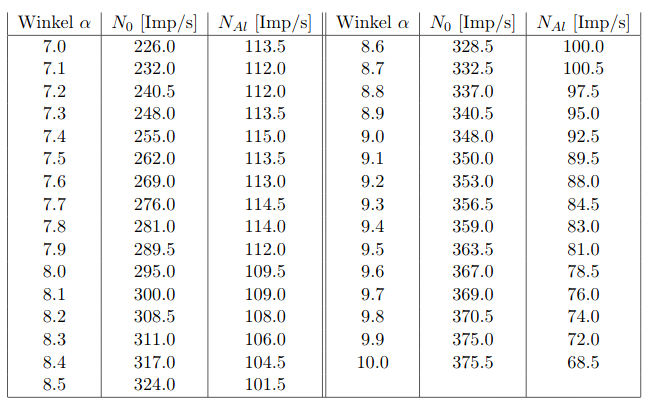
\includegraphics[width = 1.1\linewidth]{Tabelle_Transmission.png}
          \caption{Die Werte der Winkel und der zugehörigen Zählraten zu der Transmissionskurve.}
          \label{fig:transmissionstabelle}
        \end{figure}
        \FloatBarrier

        \section{Literaturverzeichnis}
        [1] \textit{Versuchsanleitung V603 - Compton-Effekt.} TU Dortmund, 2020 \newline
        [2] Physical Measurement Laboratory: \textit{X-Ray Transition Energies Database} 09.Dezember.2019
        \url{https://physics.nist.gov/PhysRefData/XrayTrans/Html/search.html}

\end{document}

